% !TEX root =  ../STVR-model-seeding.tex

%%%%%%%%%%%%%%%%%%%%%%
\section{Evaluation Results}
\label{sec:model_seeding:eval-results}
%%%%%%%%%%%%%%%%%%%%%%



We present the results of the evaluation and answer the two research questions by comparing each seeding strategy with no-seeding.
%Figure \ref{fig:eval:results} presents the general results of our evaluation per crash. In Figure \ref{fig:eval:results-crashes}, The 122 crashes (100\%) are classified for each seeding configuration of model-seeding and no-seeding according to the outcome observed in the majority of the 30 executions. The model-seeding configurations refer to the different values used for $Pr[pick\ init]  \in \{0.2, 0.5, 0.8, 1.0\} $.

%(in Figure \ref{fig:eval:results-crashes}).
%The 122 crashes (100\%) are classified for each seeding configuration according to the outcome observed in the majority of the 30 executions.
%The configurations refer to the configuration used for seeding: no seeding (no s.), test seeding with $Pr[clone] \in \{0.2, 1.0\}$ (\textit{test s.}), and behavioral model seeding with $Pr[pick\ init]  \in \{0.2, 0.5, 0.8, 1.0\} $ (\textit{model s.}).


%\begin{table} [t]
%    \centering
%	\caption{Experiment results for no seeding, test seeding, and model seeding.}
%	\label{tab:results}
%	\begin{smaller}
%	
%%%%%%%%%%%%%%%%%%%%%%%%%%%%%%%%%%%%%%%%%%
\section{Results}
\label{sec:cub:results}
%%%%%%%%%%%%%%%%%%%%%%%%%%%%%%%%%%%%%%%%%%

\begin{figure}[t]
    \centering
    \subfloat[Test cases commonality scores.]{
        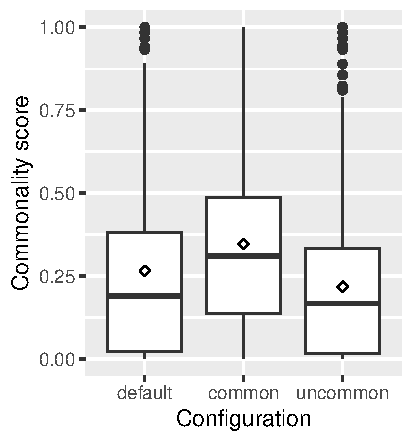
\includegraphics[height=50mm]{papers/cub/images/score.pdf}
        \label{subfig:score}
    }
    \subfloat[Effect sizes $\widehat{A}_{12}$ .]{
        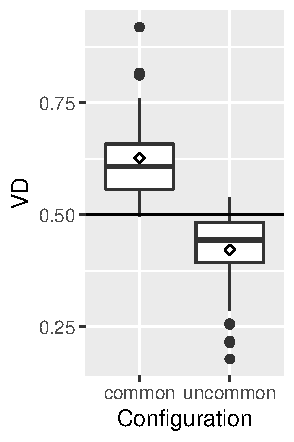
\includegraphics[height=50mm]{papers/cub/images/score-vd.pdf}
        \label{subfig:scorevd}
    }\\
    \subfloat[Effect sizes $\widehat{A}_{12}$ magnitudes.% (\textit{Significant differences $<0.05$}.
    ]{
        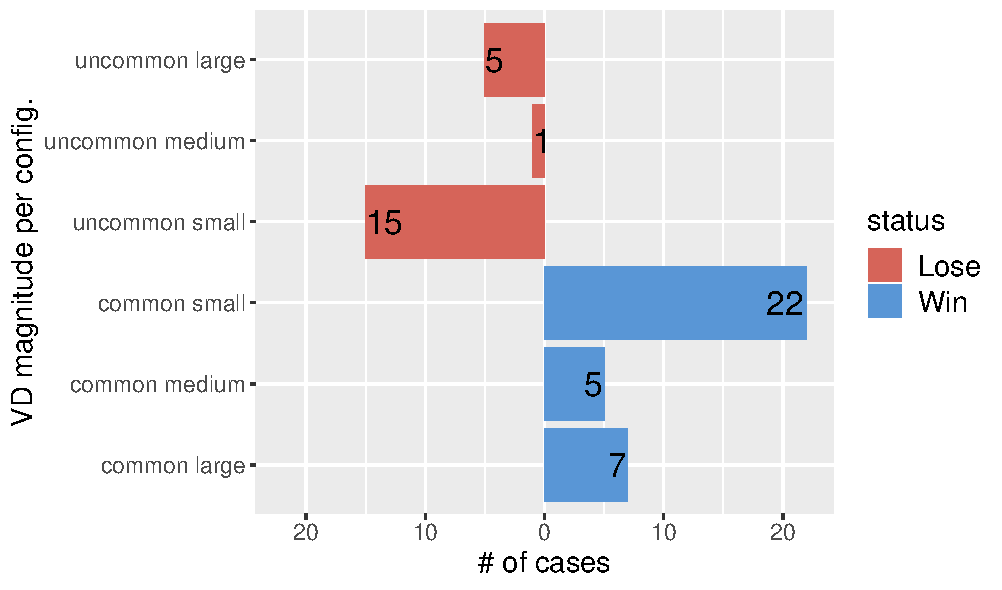
\includegraphics[height=50mm]{papers/cub/images/score-sig.pdf}
        \label{subfig:scoresig}
    } 
    
    \caption{Test cases commonality values and comparison to \df. Diamonds indicate mean values and horizontal bars (\textbf{--}) indicate median values.}
    \label{fig:rq1}
\end{figure}

\subsection{Commonality Score (RQ.1)}

In this section we answer the question: \emph{How does the \emph{commonality score} of the generated tests compare when using the \textit{common}, \textit{uncommon}, and \textit{default} secondary objectives?}

Figure \ref{fig:rq1} illustrates the impact of using \com and \ucom, as the secondary objective, on the commonality score of the generated test cases. Figure \ref{subfig:score} shows that the average and median of the commonality score is improved by 8\% and 12\%, respectively, compared to \df when using \com as secondary objective.
In parallel, using \ucom as secondary objective reduces the commonality score by, on average, 5\% (2.5\% for median) compared to \df. Moreover, Figure \ref{subfig:scoresig} presents the number of cases (\ie classes used as the target class for unit testing), in which the application of \com and \ucom significantly (\textit{p-value} $<0.05$) changes the commonality score with effect size magnitude of large, medium, or small. As we can see in this figure, utilizing \com always leads to a significant improvement in the commonality score (blue bars), and in contrast, using \ucom always reduces this score (red bars). In total, \com significantly improves the commonality score in 34 cases (32.6\% of classes), and \ucom significantly reduces this score in 21 classes (20.1\% of cases). Figure \ref{subfig:scorevd} depicts the effect sizes of differences observed in these cases. Consistent with the previous figures, the average effect size ($\widehat{A}_{12}$) achieved by \com is higher than 0.5 (\ie commonality score has been improved). However, this value is lower than 0.5 for \ucom.

\paragraph{Summary} Using \com as secondary objective in the \evosuite search-based test case generation process leads to test cases that exhibit an improved commonality score. In parallel, the application of \ucom leads to the reduction of the commonality score.

%-----------------------------------------
\subsection{Structural Coverage (RQ.2)}
%-----------------------------------------

In this section we provide an answer to the following research question: \emph{How does the \emph{line} and \emph{branch coverage} of the generated tests  compare when using the \textit{common}, \textit{uncommon}, and \textit{default} secondary objectives?}

Figure~\ref{fig:rq2} shows the line and branch coverage achieved by using \com and \ucom as secondary objectives compared to \df. Figure~\ref{subfig:coverage} indicates that the average coverage is the same for all of the assessed configurations.

Looking at the comparison of the structural coverage values achieved by each secondary objective in each class, we can see that the line and branch coverage is significantly impacted by \com and \ucom in some cases. Figure~\ref{subfig:coveragesig} presents the number of cases that these secondary objectives significantly (\textit{p-value} $<0.05$) reduce ($\widehat{A}_{12} < 0.5$) or increase ($\widehat{A}_{12} > 0.5$) the line and branch coverage with effect size magnitude small, medium, or large. According to this figure, in general, utilizing \com leads to a significant improvement for line and branch coverage in three and four classes, respectively. Nevertheless, this secondary objective reduced the line and branch coverage in eight and nine classes, respectively. 

Also, we can see a similar result for \ucom:
significant improvements in three and five classes and significant reductions in seven and nine cases for line and branch coverage. Since the number of cases in which \com and \ucom lead to a significantly lower structural coverage is higher than the the number of cases in which we see a significant improvement in coverage, the average effect size of differences (Figure~\ref{subfig:coveragevd}) is slightly less than  $0.5$ for both line (0.47 for both secondary objectives) and branch coverage (0.46 for both).

\paragraph{Summary} On average, using \com or \ucom does not impact the line and branch coverage. However, these two secondary objectives can significantly impact the structural coverage in specific cases.

\begin{figure}[t]
    \centering
    \subfloat[Test suites coverage and mutation score.]{
        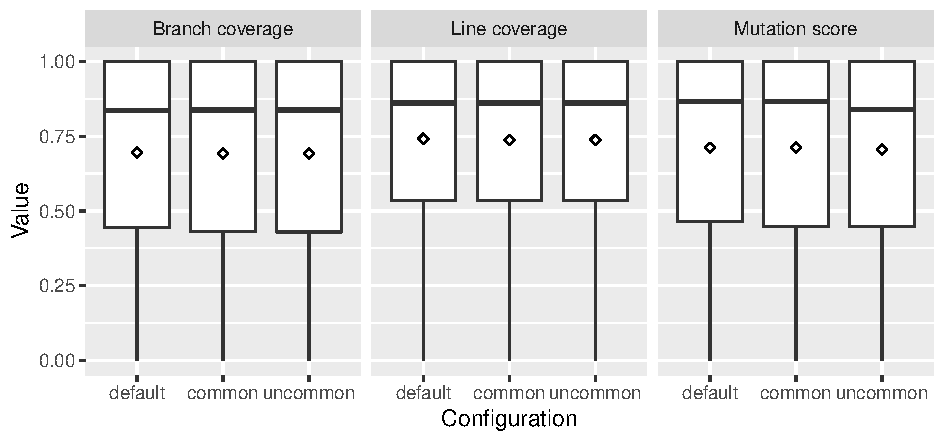
\includegraphics[height=30mm]{papers/cub/images/coverage.pdf}
        \label{subfig:coverage}
    }\hfill
    \subfloat[Effect sizes $\widehat{A}_{12}$.]{
        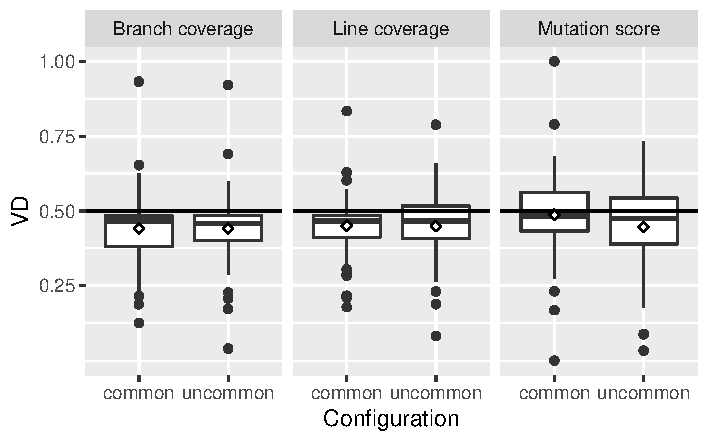
\includegraphics[height=30mm]{papers/cub/images/coverage-vd.pdf}
        \label{subfig:coveragevd}
    }\\ 
    \subfloat[Effect sizes $\widehat{A}_{12}$ magnitudes.]{
        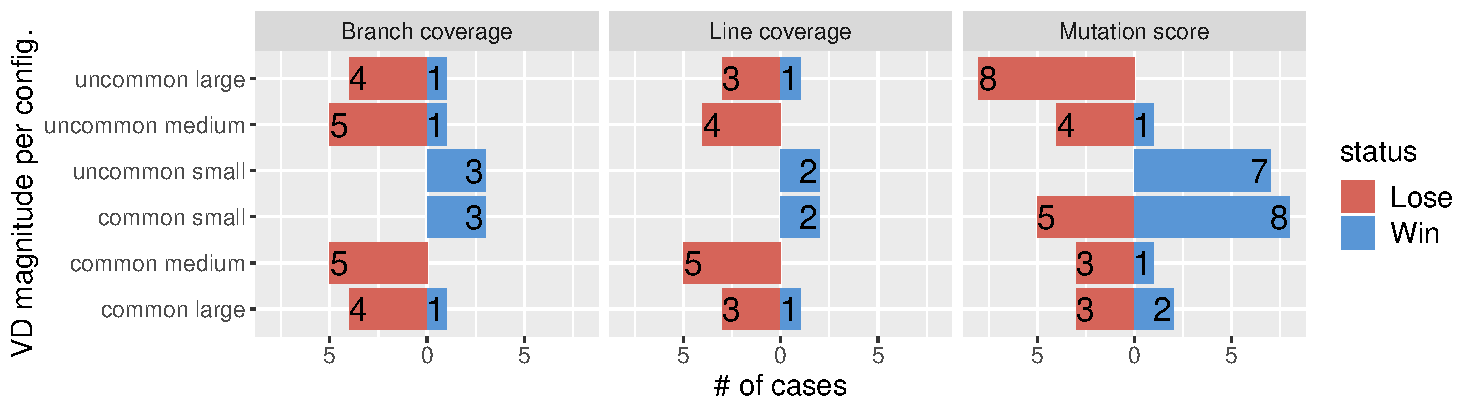
\includegraphics[height=30mm]{papers/cub/images/coverage-sig.pdf}
        \label{subfig:coveragesig}
    }
   
    \caption{Test suites coverage and mutation score, and comparison to \textit{default}. Diamonds indicate mean values and horizontal bars (\textbf{--}) indicate median values.}
    \label{fig:rq2}
\end{figure}

%-----------------------------------------
\subsection{Mutation Analysis (RQ.3)}
%-----------------------------------------

In the final research question we reflect on \emph{How does the \emph{mutation score} of the generated tests  compare when using the \textit{common}, \textit{uncommon}, and \textit{default} secondary objectives? }

Figure \ref{subfig:coverage} depicts the mutation score achieved by using \com and \ucom compared to \df. Like line and branch coverage, the average mutation scores achieved by these secondary objectives is similar to the one achieved by \df. 
However, Figure \ref{subfig:coveragesig} shows that \com and \ucom can significantly (\textit{p-value} $<0.05$) impact the mutation score achieved by unit test generation. The \com secondary objective significantly increases the number of mutants killed for 11 classes but, at the same time, also decreases the mutation score in another 11 cases. Moreover, \ucom significantly changes the mutation score in 20 cases (8 wins against 12 losses). 
Figure \ref{subfig:coveragevd} shows the effect size of differences in these cases for both \com and \ucom secondary objectives. According to this Figure, the average $\widehat{A}_{12}$ estimations are 0.49 and 0.47. Since these values are lower than 0.5, on average, the difference achieved by these two secondary objectives is negative. However, the outliers in this figure show us that the effect sizes of \com above 0.75 in some specific cases. Hence, the graphs in Figure~\ref{subfig:coveragesig} indicate that using \com and \ucom can improve the mutation score in specific cases.

\paragraph{Summary} On average, using \com or \ucom does not have any effect on the mutation score achieved by the generated test suites. However, these two secondary objectives can significantly change the killed mutants in some cases.
%	\end{smaller}
%\end{table}

%Figure \ref{fig:ffevals} presents the distribution of the number of fitness evaluations for the frames that could be reproduced by each seeding configuration in the 10 rounds of execution. The number of fitness evaluations varies between 0 (\ie the crash is reproduced by one of the test cases of the initial population) and 62,328 (\ie the maximum budget allocated for the search). For each box, we also provide the mean (represented as a white diamond) and number of observations (\ie the number of executions with a reproduction) at the top.



%--------------------------------------------------------------------------------
\subsection{Test seeding (\textbf{RQ1})}
%--------------------------------------------------------------------------------

%\item[\textbf{RQ1.1}] Can test seeding help to initialize the search process?
%\item[\textbf{RQ1.2}] Does test seeding help to replicate more crashes?
%\item[\textbf{RQ1.3}] Does test seeding impact the efficiency of the search process?
%\item[\textbf{RQ1.4}] Which factors in test seeding help the search process compared to no seeding?

\begin{table}[t]
    \center
    \caption{Odds ratios of model/test seeding configurations vs. no seeding in crash reproduction ratio. This table only shows the crashes, which reveal statistically significant differences (p-value $< 0.05$). An Odds ratio value higher than 1.0 gives that the seeding strategy is better than no seeding, and a value lower than 1.0 shows the opposite.}
	\label{tab:oddratios}
	\footnotesize
	\subfloat{\begin{tabular}{ l | l | r}
\hline 
\textbf{Conf.} & \textbf{Crash} & \textbf{Odds Ratio (p-value)} \\ 
\hline 
test s. 0.5 & LANG-6b & Inf (2.37e-02)\\ 
 & MATH-1b & 0.00 (1.69e-17)\\ 
 & MATH-61b & 0.00 (1.69e-17)\\ 
 & CHART-4b & 0.00 (1.69e-17)\\ 
 & TIME-20b & 0.00 (1.94e-03)\\ 
 & TIME-10b & 207.79 (2.36e-12)\\ 
 & TIME-5b & 3.52 (3.52e-02)\\ 
\hline 
test s. 0.8 & LANG-6b & Inf (1.94e-03)\\ 
 & MATH-1b & 0.00 (1.69e-17)\\ 
 & MATH-61b & 0.00 (1.69e-17)\\ 
 & CHART-4b & 0.00 (1.69e-17)\\ 
 & TIME-20b & 0.00 (4.64e-05)\\ 
 & TIME-10b & Inf (9.23e-14)\\ 
 & TIME-7b & 0.00 (6.19e-07)\\ 
\hline 
test s. 1.0 & LANG-51b & 0.21 (8.21e-03)\\ 
 & LANG-6b & Inf (4.64e-05)\\ 
 & MATH-1b & 0.00 (1.69e-17)\\ 
 & MATH-61b & 0.00 (1.69e-17)\\ 
 & CHART-4b & 0.00 (1.69e-17)\\ 
 & TIME-20b & 0.00 (5.83e-06)\\ 
 & TIME-10b & 69.79 (2.82e-10)\\ 
\hline 
test s. 0.2 & MATH-1b & 0.00 (1.69e-17)\\ 
 & MATH-61b & 0.00 (1.69e-17)\\ 
 & CHART-4b & 0.00 (1.69e-17)\\ 
 & TIME-20b & 0.00 (3.19e-04)\\ 
 & TIME-10b & Inf (9.23e-14)\\ 
 & TIME-7b & 0.00 (1.05e-02)\\ 
\hline 
\end{tabular}}
    \subfloat{\begin{tabular}{ l | l | r}
\hline 
\textbf{Conf.} & \textbf{Crash} & \textbf{Odds Ratio (p-value)} \\ 
\hline 
model s. 0.2 & LANG-9b & Inf (1.94e-03)\\ 
 & LANG-51b & 0.17 (3.33e-03)\\ 
 & MOCKITO-10b & Inf (1.43e-08)\\ 
 & XWIKI-13141 & 13.95 (5.58e-03)\\ 
\hline 
model s. 0.5 & LANG-9b & Inf (2.37e-02)\\ 
 & MOCKITO-10b & Inf (1.87e-07)\\ 
 & XWIKI-13141 & Inf (7.97e-04)\\ 
 & XWIKI-14152 & 6.66 (7.41e-03)\\ 
\hline 
model s. 0.8 & LANG-9b & Inf (1.94e-03)\\ 
 & LANG-51b & 0.29 (3.70e-02)\\ 
 & MOCKITO-10b & Inf (8.27e-10)\\ 
 & XWIKI-13141 & Inf (7.97e-04)\\ 
 & XWIKI-14152 & 11.24 (2.51e-04)\\ 
\hline 
model s. 1.0 & LANG-9b & Inf (1.94e-03)\\ 
 & MOCKITO-10b & Inf (5.34e-08)\\ 
 & XWIKI-13141 & 13.95 (5.58e-03)\\ 
 & XWIKI-14152 & 32.80 (5.62e-08)\\ 
\hline 
\end{tabular}}
\end{table}

\subsubsection{Crash reproduction effectiveness (\textbf{RQ1.1})}

Figure~\ref{fig:eval:results} demonstrates the comparison of each seeding strategy (left-side of the figure is for test seeding and right-side is for model seeding) with the baseline (no seeding). Figures~\ref{fig:eval:results-rq12} and \ref{fig:eval:results-rq22} show the overall comparison, while Figures~\ref{fig:eval:results-rq12-apps} and~\ref{fig:eval:results-rq22-apps} illustrate the per project comparison. In each of these figures, the yellow bar shows the number of reproduced crashes in the majority of the 30 executions, and the orange bar shows the non-reproduced crashes.

According to Figure \ref{fig:eval:results-rq12}, \textit{test s. 0.8} reproduced the same number of crashes. However, the other configurations of test-seeding reproduced fewer crashes in the majority of times. Moreover, according to Figure \ref{fig:eval:results-rq12-apps}, test seeding reproduces one more crash compared to no seeding. Also, some configurations of test seeding can reproduce one extra crash in  XWiki and commons-lang projects. On the contrary, all of the configurations of test seeding missed one and two crashes in JFreeChart and commons-math, respectively. Finally, we cannot see any difference between test seeding and no seeding in the Joda-Time project.
 
 
 %Each of the observed differences in this figure is manually analyzed.
 %The observed factors in the manual analysis will be discussed in Section \ref{sec:eval:rq14}.

Table \ref{tab:crash-repr-table} demonstrates the impact of test-seeding on the crash reproduction ratio compared to no-seeding. It indicates that \textit{test s. 0.2 \& 0.5} have a better crash reproduction ratio for one of the crashes, while they perform significantly worse in 4 other crashes compared to no-seeding. The situation is almost the same for the other configurations of test seeding: \textit{test s. 0.8 \& 1.0} are significantly better in 2 crashes compared to no-seeding. However, they are significantly worse than no-seeding in 5 other crashes. The other interesting point in this table is the standard deviation crash reproduction ratio. This value is slightly higher for all of the test seeding configurations compared to no seeding. The values of odds ratios and and p-values for crashes with significant difference is available in Table \ref{tab:oddratios}.
%The cases which make the difference in this table are included in the manual analysis for Section \ref{sec:eval:rq14}.
%Table \ref{tab:reproduction-ranking} ranks the different configurations regarding their crash reproduction capability (\textbf{RQ1.2}). Only \textit{test s. 0.2} ranks better than no seeding, but not significantly. All other configurations are not significantly worse. Only test seeding with \textit{test s. 0.2} performs significantly better than \textit{test s. 0.5} and \textit{test s. 1.0}.

The underlying reasons for the observed results in this section are analyzed in \textbf{RQ1.4}.
\begin{figure*}[t]
	\centering
	\subfloat[test-seeding vs. no-seeding (for all projects together)]{
		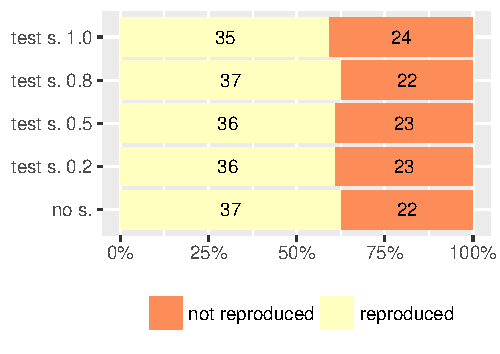
\includegraphics[height=40mm]{papers/model_seeding/figures/evaluation/rq12-crashes-all.pdf}
		\label{fig:eval:results-rq12}
	}\hfill  
	\subfloat[model-seeding vs. no-seeding (for all projects together)]{
		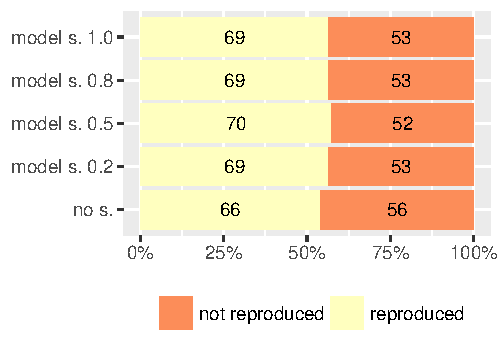
\includegraphics[height=40mm]{papers/model_seeding/figures/evaluation/rq22-crashes-all.pdf}
		\label{fig:eval:results-rq22}
	}

\subfloat[test-seeding vs. no-seeding (per project)]{
	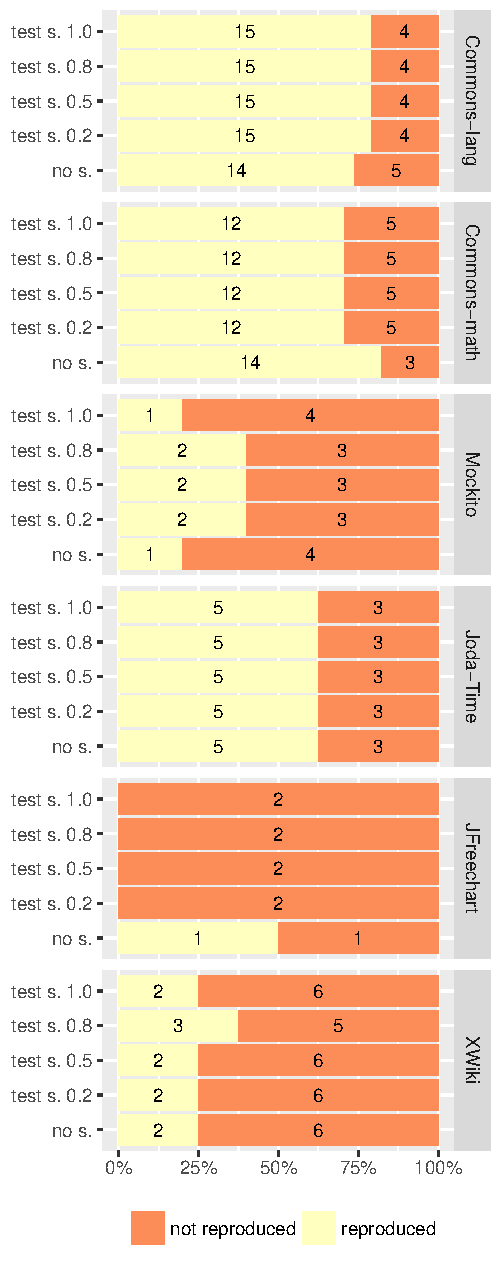
\includegraphics[height=130mm]{papers/model_seeding/figures/evaluation/rq12-crashes-apps.pdf}
%	    \vspace{-1mm}
	% \caption{test-seeding vs. no-seeding (per project)}
	\label{fig:eval:results-rq12-apps}
}\hfill
\subfloat[model-seeding vs. no-seeding (per project)]{
	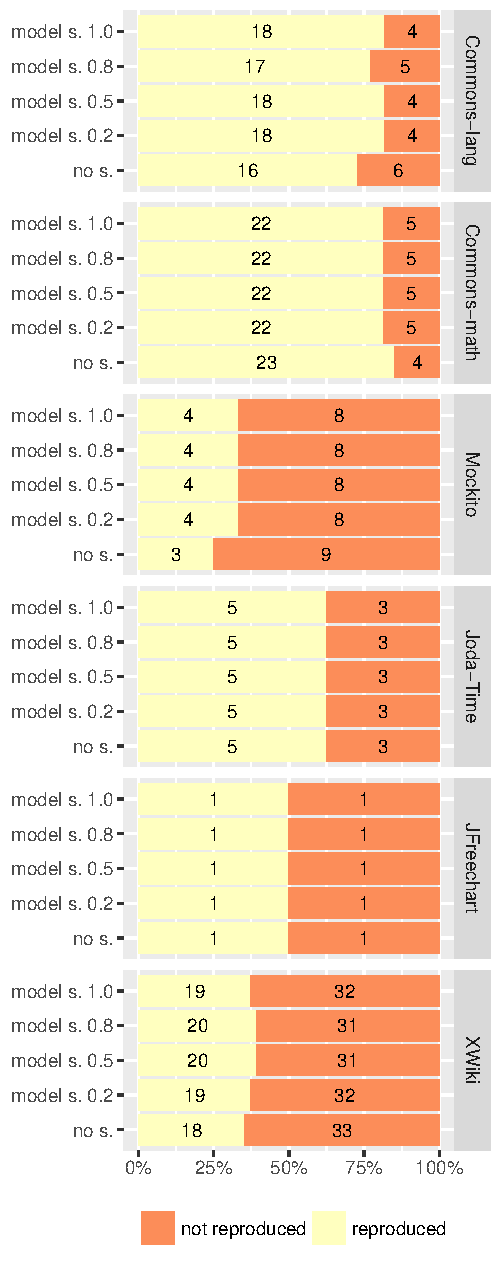
\includegraphics[height=130mm]{papers/model_seeding/figures/evaluation/rq22-crashes-apps.pdf}
%	    \vspace{-1mm}
	% \caption{test-seeding vs. no-seeding (per project)}
	\label{fig:eval:results-rq22-apps}
}
   \vspace{-3mm}
	\caption{Outcomes observed in the majority of the executions for each crash in total and for each application.}
%	\label{fig:eval:resultsdetails}
	\label{fig:eval:results}
\end{figure*}


\begin{table} [t]
	\center
	\caption{Evaluation results for comparing seeding strategies (test and model seeding) and no-seeding in crash reproduction. $\overline{\text{ratio}}$ and $\sigma$  designate average crash reproduction ratio and standard deviation, respectively. The numbers in the comparison only count the statistically significant cases.}
	\label{tab:crash-repr-table}
%	\vspace{-2mm}
	\begin{footnotesize}
	\subfloat{\begin{tabular}{ l r r | r r r }
  \hline 
  \textbf{Conf.} & \multicolumn{2}{c|}{Reproduction} & \multicolumn{2}{c}{Comparison to no s.} \\ 
    & $\overline{\text{ratio}}$ & $\sigma$ & better & worse \\ 
  \hline 
  test s. 1.0 & 23.7 & 11.01 & 2 & 5 \\ 
  test s. 0.8 & 23.4 & 10.74 & 2 & 5 \\ 
  test s. 0.5 & 23.8 & 10.76 & 1 & 4 \\ 
  test s. 0.2 & 23.5 & 10.93 & 1 & 4 \\ 
  no s. & 25.4 & 9.65 & - & - \\ 
  \hline 
  \end{tabular}}
	\subfloat{\begin{tabular}{ l r r | r r r }
\hline 
\textbf{Conf.} & \multicolumn{2}{c|}{Reproduction} & \multicolumn{2}{c}{Comparison to no s.} \\ 
  & $\overline{\text{ratio}}$ & $\sigma$ & better & worse \\ 
\hline 
model s. 1.0 & 22.0 & 11.58 & 4 & 0 \\ 
model s. 0.8 & 21.9 & 11.92 & 4 & 1 \\ 
model s. 0.5 & 21.8 & 11.86 & 4 & 0 \\ 
model s. 0.2 & 21.6 & 12.00 & 3 & 1 \\ 
no s. & 21.3 & 12.32 & - & - \\ 
\hline 
\end{tabular}}
	
    \end{footnotesize}
%	\vspace{-3mm}
\end{table}

\subsubsection{Crash reproduction efficiency (\textbf{RQ1.2})}

Table \ref{tab:fitness-evaluation-table} demonstrates the comparison of test-seeding and no-seeding in the number of needed fitness function evaluations for crash reproduction. The average number of fitness function evaluations increases when using test-seeding. It means that test-seeding is slower than no-seeding on average. \textit{test s. 0.8} has the highest average fitness function evaluations. 

Moreover, the standard deviations of both no seeding and test seeding are high values (more than 20k evaluations). This notable variation is explainable due to the nature of search-based approaches. In some executions, the initialized population is closer to the objectives, and the search process can achieve reproduction faster. Similar variations are reported in the \jcrashpack empirical evaluation as well (Chapter 2). According to the reported standard deviations, we can see that this value increases for all of the configurations of test seeding compared to no seeding.

Also, the values of the effect sizes indicate that the number of crashes that receive (large or medium) positive impacts from \textit{test s. 0.2 \& 0.5} for their reproduction speed is higher than the number of crashes that exhibit a negative (large or medium) influence. However, this is not the case for the other two configurations. In the worst case, \textit{test s. 1.0} is considerably slower than no-seeding (with large effect size)  in 13 crashes.


\begin{table*} [t]
	\center
	\caption{Evaluation results for comparing test-seeding and no-seeding in the number of fitness evaluations $\overline{\text{evaluations}}$ and $\sigma$  designate average fitness function evaluations needed for crash reproduction and standard deviation, respectively. The numbers in the comparison only count the statistically significant cases.}
%	\vspace{-2mm}
	\label{tab:fitness-evaluation-table}
	\begin{footnotesize}
	\begin{tabular}{ l r r | rr | rr | rr }
\hline 
\textbf{Conf.} & \multicolumn{2}{c|}{Fitness} & \multicolumn{6}{c}{Comparison to no s.} \\ 
  &   &   & \multicolumn{2}{c}{large} & \multicolumn{2}{c}{medium} & \multicolumn{2}{c}{small} \\ 
  & $\overline{\text{evaluations}}$ & $\sigma$ & $<0.5$ & $>0.5$ & $<0.5$ & $>0.5$ & $<0.5$ & $>0.5$ \\ 
\hline 
no s. & 10,467 & 22,368.13 & - & - & - & - & - & - \\ 
test s. 0.2 & 14,089 & 25,464& 4& 3& 1& 1& 2& - \\ 
test s. 0.5 & 13,366 & 25,043& 5& 3& 1& -& 2& 1 \\ 
test s. 0.8 & 14,254 & 25,496& 3& 4& 1& 5& 1& 3 \\ 
test s. 1.0 & 13,856 & 25,097& 3& 13& 4& 3& 1& 3 \\ 
\hline 
\end{tabular}
	\end{footnotesize}
%	\vspace{-3mm}
\end{table*}



\subsubsection{Guided initialization effectiveness (\textbf{RQ1.3})}

Table \ref{tab:starting-effect-size} indicates the number of crashes where test-seeding had a significant (p-value $< 0.05$) impact on the search initialization compared to no-seeding. As we can see in this table, any configuration of test-seeding has a negative impact on the search starting process for 4 or 5 crashes. Additionally, this strategy does not have any significant beneficial impact on this aspect except on one crash in \textit{test s. 0.8}. Also, the standard deviation of the average search initialization ratios, in all of the configurations of test seeding, is increased compared to no seeding. For instance, this value for \textit{test s. 0.8} is about three times more than no seeding.


\begin{table}[t]
	\center
	\caption{Evaluation results for comparing seeding strategies (test and model seeding) and no-seeding in search initialization. $\overline{\text{ratio}}$ and $\sigma$  designate average successful search initialization ratio and standard deviation, respectively. The numbers in the comparison only count the statistically significant cases.}
	\label{tab:starting-effect-size}
%	\vspace{-2mm}
	\begin{footnotesize}
		\subfloat{\begin{tabular}{ l r r | r r r }
\hline 
\textbf{Conf.} & \multicolumn{2}{c|}{Search started} & \multicolumn{2}{c}{Comparison to no s.} \\ 
  & $\overline{\text{ratio}}$ & $\sigma$ & better & worse \\ 
\hline 
test s. 1.0 & 26.9 & 9.22 & 0 & 5 \\ 
test s. 0.8 & 27.9 & 7.67 & 1 & 4 \\ 
test s. 0.5 & 26.9 & 9.22 & 0 & 5 \\ 
test s. 0.2 & 27.4 & 8.49 & 0 & 4 \\ 
no s. & 29.5 & 3.94 & - & - \\ 
\hline 
\end{tabular}}
		\subfloat{\begin{tabular}{ l r r | r r r }
\hline 
\textbf{Conf.} & \multicolumn{2}{c|}{Search started} & \multicolumn{2}{c}{Comparison to no s.} \\ 
  & $\overline{\text{ratio}}$ & $\sigma$ & better & worse \\ 
\hline 
model s. 1.0 & 30.0 & 0.28 & 3 & 0 \\ 
model s. 0.8 & 30.0 & 0.00 & 3 & 0 \\
model s. 0.5 & 29.7 & 2.75 & 2 & 0 \\ 
model s. 0.2 & 29.5 & 3.87 & 2 & 1 \\
no s. & 29.2 & 4.72 & - & - \\ 
\hline 
\end{tabular}}
	\end{footnotesize}
%	\vspace{-3mm}
\end{table}


\subsubsection{Influencing factors (\textbf{RQ1.4})}
\label{sec:eval:rq14}

To finding the influencing factors in test seeding, we manually analyzed the cases which cause significant differences, in various aspects, between no-seeding and test-seeding. From our manual analysis, we identified 3 factors of the test seeding process that influence the search:
%
\begin{inparaenum}[(i)]
\item \textbf{Crash-Test Proximity},
\item \textbf{Crash-Object Proximity}, and
\item \textbf{Test Execution Cost}.
\end{inparaenum}

\paragraph{Crash-Test Proximity} For the first factor, we observe that \emph{cloning existing test cases} in the initial population leads to \emph{the reproduction of new crashes} when the cloned tests include elements which are close to the crash reproducing test. For instance, all of the configurations of test seeding are capable of reproducing the crash LANG 6b, while no-seeding cannot reproduce it. For reproducing this crash, Botsing needs to generate a string of a specific format, and this format is available in the existing test cases, which are seeded to the search process.

However, manually developed tests are not always helpful for crash reproduction. According to the results of Table \ref{tab:fitness-evaluation-table}, \textit{test s. 1.0}, which always clones test cases, is considerably and largely slower than no-seeding in 13 crashes. In these cases, cloning all of the test cases to form the initial population can prevent the search process from reaching the crash reproducing test. As an example, Botsing needs to generate a simple test case, which calls the target method with an empty string and null object, to reproduce crash LANG-12b. But, \textit{test s. 1.0} clones tests which use the software under test in different ways.
To summarize, the overall quality of results of our test seeding solution is highly dependent on the quality of the existing test cases in terms of factors like the distance of existing test cases to the scenario(s) in which the crash occurs and the variety of input data.


\paragraph{Crash-Object Proximity} For the second factor, we observe that (despite the fixed value of $Pr[pick\ mut]$ for test seeding), the objects with call sequences carved from the existing tests and stored in the object pool can help during the search depending on their diversity and their distance from the call sequences that we need for reproducing the given crash. For instance, for crash MATH-4b, \botsing needs to initialize a \texttt{List} object with at least two elements before calling the target method in order to reproduce the crash. In test-seeding, such an object had been carved from the existing tests and allowed test seeding to reproduce the crash faster. Also, test-seeding can replicate this crash more frequently: the number of successfully replicated executions, in 30 runs, is higher with test-seeding.

In contrast, the carved objects can misguide the search process for some crashes which need another kind of call sequence.  For instance, in crash MOCKITO-9b, Botsing cannot inject the target method into the generated test because the carved objects do not have the proper state to instantiate the input parameters of the target method.

In summary, if the involved classes in a given crash are well-tested (the existing tests contain all of the usage scenarios of these classes), we have more chances to reproduce by utilizing test-seeding.


\paragraph{Test Execution Cost} The third factor points to the challenge of executing the existing test cases for seeding. The related tests for some crashes are either expensive (time/resource consuming) or challenging (due to the security issues) to execute. Hence, the \evosuite test executor, which is used by Botsing, cannot carve all of them. 

As an example of expensive execution, the EvoSuite test executor spends more than 1 hour during the execution of the related test cases for replicating frame 2 of crash Math-1b.

Also, as an example for security issues, the EvoSuite test executor is not successful in running some of the existing tests. It throws an exception during this task. For instance, this executor throws \texttt{java.lang.SecurityException} during the execution of the existing test cases for CHART-4b, and it cannot carve any object for seeding.

In some cases, test-seeding faces the mentioned problems during the execution of all of the existing test cases for a crash. If test seeding cannot carve any object from existing tests, there will be no useful call sequence in the object pool to seed during the search process. Hence, although the project contains some potentially valuable test scenarios for reproducing the given crash, there is no difference between no seeding and test seeding in these cases.
%\andy{This last point is too abstract for me to comprehend... I need more to really see the deeper issue... sorry!
%\pouria{I rewrote the ``Expensive test execution for collecting tests"}
%}


%\begin{lstlisting}[basicstyle=\scriptsize\ttfamily,
%breaklines=true,
%numbers=left,
%xleftmargin=2em,
%frame=top,frame=bottom,
%caption={A sample of an existing test in java commons math},
%label=lst:existing-test,
%float=t]
%@Test
%public void test0() {
%  ...
%  List<double[]> threeClasses = new ArrayList<>();
%  threeClasses.add(classA);
%  threeClasses.add(classB);
%  threeClasses.add(classC);
%  ...
%}
%\end{lstlisting}

\subsubsection{Summary (\textbf{RQ1)}}

Test seeding (for any configuration) loses against no-seeding in the search initialization because some of the related test cases of crashes are expensive or even impossible to execute.
Also, we observe in the manual analysis that the lack of generality in the existing test cases prevents the crash reproduction search process initialization. In these cases, the carved objects from the existing tests mismatch the search process in the target method injection.
% \andy{Previous sentence too vague... especially the word ``tricky''... it is not so much about tricky if I understand correctly, but about the quality of existing test cases? \pouria{I rephrased it.}}
Moreover, this seeding strategy can outperform no seeding in the crash reproduction and search efficiency for some cases (\eg LANG 6b), thanks to the call sequences carved from the existing tests. However, these carved call sequences can be detrimental to the search process in some cases, if the carved call sequences do not contain beneficial knowledge about crash reproduction, overusing them can misguide the search process.


%--------------------------------------------------------------------------------
\subsection{Behavioral model seeding (\textbf{RQ2})}
%--------------------------------------------------------------------------------



\subsubsection{Crash reproduction effectiveness (\textbf{RQ2.1})}

Figure~\ref{fig:eval:results-rq22} draws a comparison between model-seeding and no-seeding in the crash reproduction ratio according to the results of the evaluation on all of the 122 crashes. As mentioned in Section~\ref{sec:setup:setup:selection}, since model seeding collects call sequences both from source code and existing tests, it can be applied to all of the crashes (even the crashes that do not have any helpful test). As depicted in this Figure, all of the configurations of model-seeding reproduce more crashes compared to no-seeding in the majority of runs. We observe that \textit{model s. 0.2 \& 0.5 \& 1.0} reproduce 3 more crashes than no-seeding. In addition, in the best performance of model-seeding, \textit{model s. 0.8} reproduces 70 out of 122 crashes (6\% more than no-seeding).


Figure~\ref{fig:eval:results-rq22-apps} categorizes the results of Figure~\ref{fig:eval:results-rq22} per application. As we can see in this figure, model seeding replicates more crashes for XWiki, commons-lang, and Mockito. However, no-seeding reproduces one crash more than model-seeding for commons-math. For the other projects, the number of reproduced crashes does not change between no-seeding and different configurations of model-seeding. 

We also check how many crashes can be reproduced at least once with model seeding, but not with no seeding. In total, model-seeding configurations reproduce nine new crashes that no-seeding cannot reproduce.

Table \ref{tab:crash-repr-table} indicates the impact of model-seeding on the crash reproduction ratio. As we can see in this table, \textit{model s. 0.2} has a significantly better crash reproduction ratio in 3 crashes. Also, other configurations of model-seeding are significantly better than no seeding in 4 crashes. This improvement is achieved by model-seeding, while 2 out of 4 configurations of model-seeding have a significant unfavorable impact on only one crash. The values of odds ratios and and p-values for crashes with significant difference is available in Table \ref{tab:oddratios}.


% \begin{table} [t]
% 	\center
% 	\caption{Evaluation results for comparing model-seeding and no-seeding in crash reproduction. $\overline{\text{ratio}}$ and $\sigma$  designate average crash reproduction ratio and standard deviation, respectively. The numbers in the comparison only count the statistically significant cases.}
% 	\label{tab:crash-repr-table-rq22}
% %	\vspace{-2mm}
% 	\begin{footnotesize}
% 	\begin{tabular}{ l r r | r r r }
\hline 
\textbf{Conf.} & \multicolumn{2}{c|}{Reproduction} & \multicolumn{2}{c}{Comparison to no s.} \\ 
  & $\overline{\text{ratio}}$ & $\sigma$ & better & worse \\ 
\hline 
model s. 1.0 & 22.0 & 11.58 & 4 & 0 \\ 
model s. 0.8 & 21.9 & 11.92 & 4 & 1 \\ 
model s. 0.5 & 21.8 & 11.86 & 4 & 0 \\ 
model s. 0.2 & 21.6 & 12.00 & 3 & 1 \\ 
no s. & 21.3 & 12.32 & - & - \\ 
\hline 
\end{tabular}
% 	\end{footnotesize}
% %	\vspace{-3mm}
% \end{table}

\subsubsection{Crash reproduction efficiency (\textbf{RQ2.2})}

Table \ref{tab:fitness-evaluation-table-rq23} compares the  number of the needed fitness function evaluations for crash reproduction in model-seeding and no-seeding. As we can see in this table, the average effort is reduced by using model-seeding. On average \textit{mode s. 1.0} achieves the fastest crash reproduction.


According to this table, and in contrast to test-seeding, model-seeding's efficiency is slightly positive. The number of crashes that model-seeding has a positive large or medium influence (as Vargha-Delaney measures are lower than 0.5) on varies between 3 to 5.
%\andy{Can a reviewer argue that we have not taken the cost of model seeding into account when determining efficiency. Is this something that we need to come back to?
%\pouria{I added a paragraph in ``data analysis procedure" (Section 6.2) to answer this question before results. }
%}
Also, model-seeding has a large adverse effect size (as Vargha-Delaney measures are higher than 0.5) on one crash, while this number is higher for test-seeding (\eg 13 for \textit{test s. 1.0}).
\begin{table*} [t]
	\center
	\caption{Evaluation results for comparing model-seeding and no-seeding in the number of fitness evaluations $\overline{\text{evaluations}}$ and $\sigma$  designate average fitness function evaluations needed for crash reproduction and standard deviation, respectively. The numbers in the comparison only count the statistically significant cases.}
%	\vspace{-2mm}
	\label{tab:fitness-evaluation-table-rq23}
	\begin{footnotesize}
	\begin{tabular}{ l r r | rr | rr | rr }
\hline 
\textbf{Conf.} & \multicolumn{2}{c|}{Fitness} & \multicolumn{6}{c}{Comparison to no s.} \\ 
  &   &   & \multicolumn{2}{c}{large} & \multicolumn{2}{c}{medium} & \multicolumn{2}{c}{small} \\ 
  & $\overline{\text{evaluations}}$ & $\sigma$ & $<0.5$ & $>0.5$ & $<0.5$ & $>0.5$ & $<0.5$ & $>0.5$ \\ 
\hline 
no s. & 18,713.1 & 28,023.93 & - & - & - & - & - & - \\ 
model s. 0.2 & 18,016.1 & 27,699.61& 2& 1& 1& 1& 2& 1 \\ 
model s. 0.5 & 17,646.9 & 27,463.02& 2& 1& 2& -& 2& 1 \\ 
model s. 0.8 & 17,564.5 & 27,400.27& 3& 1& 2& -& 1& 3 \\ 
model s. 1.0 & 17,268.8 & 27,190.73& 3& 1& 2& -& 1& 2 \\ 
\hline 
\end{tabular}
	\end{footnotesize}
%	\vspace{-3mm}
\end{table*}
Table \ref{tab:fitness-evaluation-table-rq23} does not include the cost of model generation for seeding as mentioned in our experimental setup. In our case, model generation was not a burden and is performed only once per case study. We will cover this point in more detail in Section \ref{sec:model_seeding:discussion}.    




\subsubsection{Guided initialization effectiveness (\textbf{RQ2.3})}

Table \ref{tab:starting-effect-size}  provides a comparison between model-seeding and no-seeding in the search initialization ratio. As shown in this Table, \textit{model s. 0.2 \& 0.5} significantly outperform no seeding in starting the search process for two crashes. This number increases to 3 for \textit{model s. 0.8 \& 1.0}. In contrast to test-seeding, most of the configurations of model-seeding do not have any significant negative impact on the search initialization (only \textit{model s. 0.2} is significantly worse than no-seeding in one crash). Notably, the average search initialization ratios for all of the model seeding configurations are slightly higher than no seeding. In the best case for model seeding, \textit{model s. 0.8 \& 1.0} is 30/30 runs, and the standard deviations for these two configurations are 0 or close to 0.

% \begin{table}[t]
% 	\center
% 	\caption{Evaluation results for comparing model-seeding and no-seeding in search initialization. $\overline{\text{ratio}}$ and $\sigma$  designate average successful search initialization ratio and standard deviation, respectively. The numbers in the comparison only count the statistically significant cases.}
% 	\label{tab:starting-effect-size-rq21}
% %	\vspace{-2mm}
% 	\begin{footnotesize}
% 	\begin{tabular}{ l r r | r r r }
\hline 
\textbf{Conf.} & \multicolumn{2}{c|}{Search started} & \multicolumn{2}{c}{Comparison to no s.} \\ 
  & $\overline{\text{ratio}}$ & $\sigma$ & better & worse \\ 
\hline 
model s. 1.0 & 30.0 & 0.28 & 3 & 0 \\ 
model s. 0.8 & 30.0 & 0.00 & 3 & 0 \\
model s. 0.5 & 29.7 & 2.75 & 2 & 0 \\ 
model s. 0.2 & 29.5 & 3.87 & 2 & 1 \\
no s. & 29.2 & 4.72 & - & - \\ 
\hline 
\end{tabular}
% 	\end{footnotesize}
% %	\vspace{-3mm}
% \end{table}

\subsubsection{Influencing factors (\textbf{RQ2.4})}

We have manually analyzed the crashes which lead to significant differences between different configurations of model seeding and no seeding. In doing so, we have identified 4 influencing factors in model-seeding on search-based crash reproduction, namely:
%
\begin{inparaenum}[(i)]
\item using \textbf{Call sequence dissimilarity} for guided initialization,
\item having \textbf{Information source diversity} to infer the behavioral models,
\item \textbf{Sequence priority} for seeding by focusing on the classes involved in the stack trace, and
\item having \textbf{Fixed size abstract object behavior selection} from usage models.
\end{inparaenum}

\paragraph{Call sequence dissimilarity}
Using \emph{dissimilar call sequences} to populate the object pool in model seeding seems particularly useful for search efficiency compared to test seeding. In particular, if the number of test cases is large, model seeding enables (re)capturing the behavior of those tests in the model and regenerate a smaller set of call sequences which maximize diversity, augmenting the probability to have more diverse objects used during the initialization. For instance, Botsing with model-seeding is statistically more efficient than other strategies for replicating crash XWIKI-13141. Through our manual analysis we observed that model-seeding could replicate crash XWIKI-13141 in the initial population in 100\% of cases, while the other seeding strategies replicate it after a couple of iterations. In this case, despite the large size of the target class behavioral model  (35 transitions and 17 states), the diversity of the selected abstract object behaviors guarantees that Botsing seeds the reproducing test cases to the initial population.

\paragraph{Information source diversity}
Having \emph{multiple sources} to infer the model from helps to select diversified call sequences compared to test seeding. For instance, the sixth frame of the crash XWIKI-14556 points to a class called \texttt{HqlQueryExecutor}. No seeding cannot replicate this crash because it does not have any guidance from existing solutions. Also, since the test carver could not detect any existing test which is using the related classes, this seeding strategy does not have any knowledge to achieve reproduction. In contrast, the knowledge required for reproducing this crash is available in the source code, and model-seeding learned it from static analysis of this resource. Hence, this seeding strategy is successful in accomplishing crash reproduction.

\paragraph{Sequence priority}
By \emph{prioritizing classes} involved in the stack trace for the abstract object behaviors selection, the object pool contains more objects likely to help to reproduce the crash. For instance, for the 10th frame of the crash LANG-9b, model seeding could achieve reproduction in the majority of runs, compared to 0 for test and no seeding, by using the class \texttt{Fast\-Date\-Parser} appearing in the stack trace.

\paragraph{Fixed size abstract object behavior selection}
The last factor points to the fixed number of the generated abstract object behaviors from each model. In some cases, we observed that model-seeding was not successful in crash reproduction because the usage models of the related classes were large, and it was impossible to cover all of the paths with 100 abstract object behaviors. As such, this seeding strategy missed the useful dissimilar paths in the model. As an example, model-seeding was not successful in replicating crash XWIKI-8281 (which is replicated by no-seeding and test-seeding). In this crash, the unfavorable generated abstract object behaviors for the target class misguided the search process in model seeding.

%\begin{lstlisting}[basicstyle=\scriptsize\ttfamily,
%breaklines=true,
%numbers=left,
%xleftmargin=2em,
%frame=top,frame=bottom,
%caption={A sample for a generated test for reproducing XWIKI-13372 by using model seeding},
%label=lst:xwiki-13372-reproduction,
%float=t]
%@Test
%public void test0() {
%  BaseObject baseObject0 = new BaseObject();
%  baseObject0.setLargeStringValue("", "");
%  BaseObject baseObject1 = new BaseObject();
%  baseObject1.setIntValue("}XG^cs] /4l", (-1));
%  baseObject0.equals(baseObject1);
%}
%\end{lstlisting}

\subsubsection{Summary (\textbf{RQ2})}


Model seeding achieves a better search initialization ratio compared to no seeding. With respect to the best achievement of model seeding (\textit{model s. 0.8 \& 1.0}), they decrease the number of not started searches in 3 crashes.
%
Moreover, compared to no seeding, model seeding increases the number of crashes that can be reproduced in the majority of times to 6\%. It also reproduces 9 (out of 122) extra crashes that are unreproducible with no-seeding. 
%
In addition, model seeding improves the efficiency of search-based crash reproduction compared to no seeding. It takes, on average, less fitness function evaluations. Also, model seeding delivers more positive significant impact on the efficiency of the search process compared to no seeding.
%

In general, model seeding outperforms no seeding in all of the aspects of search-based crash reproduction. According to the manual analysis that we have performed in this study, model seeding achieves this performance thanks to multiple factors: Call sequence dissimilarity, Information source diversity, and Sequence priority. Nevertheless, we observe a negative impacting factor in model seeding, as well. This factor is the fixed size abstract object behavior selection.

